\chapter{Ground Vibration Testing}
\label{ch:gvt}

Ground vibration testing (GVT) was performed to validate the preliminary finite-element model of MARGE. The frequency responses of accelerometers to an impulse input were generated from the experimental data. Using these, the natural frequencies and the damping ratios of dynamic modes of the system were determined.

Two sets of data were collected. The first set of data was collected with MARGE as designed, including the rigid-body pitching mode. This data was used to determine the damping ratios of the modes. The second set of data was collected with the root of the MARGE wing clamped to eliminate the rotational rigid-body mode. This was done to enable data acquisition of flexible-body modes without exciting and losing energy to the rigid-body mode. This data was used to tune the finite-element model and to determine the damping ratios of the wing bending modes.

%%%%%%%%%%%%%%%%%%%%%%%%%%%%%%%%%%%%%%%%%%%%%%%%%%%%%%%%%%%%%%%%
\section{Test Setup} %%%%%%%%%%%%%%%%%%%%%%%%%%%%%%%%%%%%%%%%%%%
%%%%%%%%%%%%%%%%%%%%%%%%%%%%%%%%%%%%%%%%%%%%%%%%%%%%%%%%%%%%%%%%

The equipment used for the test include:
\begin{itemize}
    \item PCB Piezotronics ICP Impact Hammer Model 086C03
    \item PCB Piezotronics ICP Accelerometer Model 352C22
    \item National Instruments Breakout <insert>
    \item National Instruments DAQ Module <insert>
\end{itemize}

The impact hammer and accelerometers were connected to the DAQ system which was connected to a personal computer. The computer recorded data from the DAQ system using the Data Acquisition Toolbox for MATLAB.

%---------------------------------------------------------------
\subsection{Sensor Placement}
%---------------------------------------------------------------

The accelerometers were placed in locations such that all of the flexible natural modes of interest were observable. This was done by placing accelerometers near anti-nodal points of the natural modes as predicted by the preliminary finite-element model. The accelerometer locations for the two sets of testing are shown in Fig. \ref{fig:accelPlacement}. The impact hammer hits were also placed at these same locations on the structure as the accelerometers.

\begin{figure}[h]
    \centering
    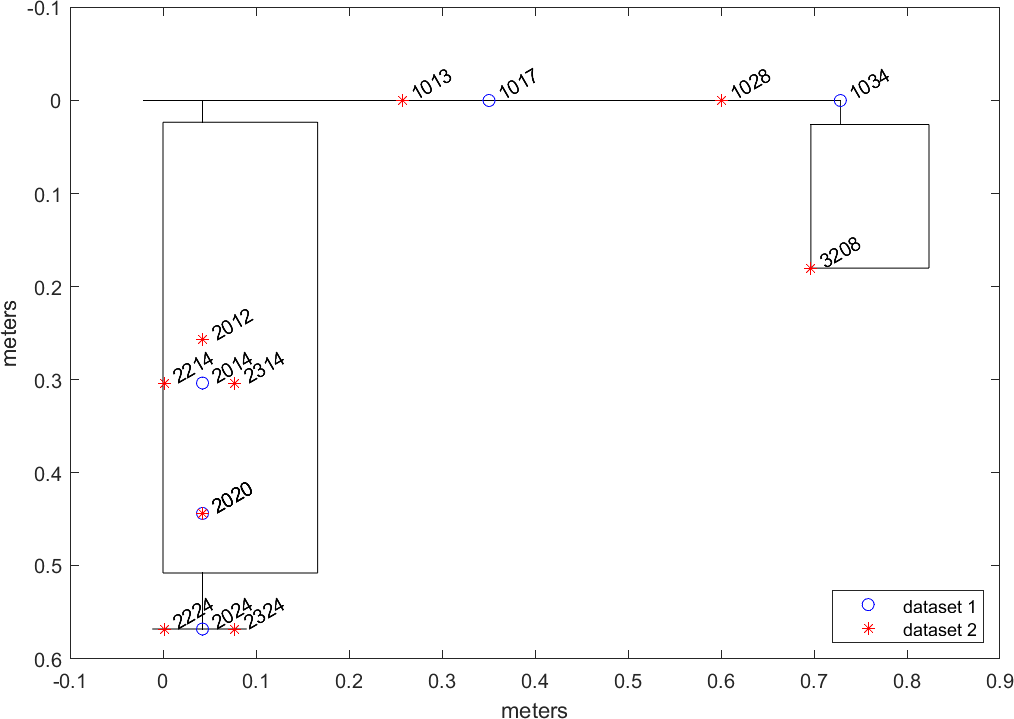
\includegraphics[width=4in]{figs/GVT/accelLocPlot.png}
    \caption{Accelerometer placement in ground vibration testing of MARGE}
    \label{fig:accelPlacement}
\end{figure}

For the second dataset, pairs of accelerometers on the wing located a short distance apart chordwise were also treated as a fictional third accelerometer by taking the difference of their signals. This was done to simulate a sensor observing only torsional modes of the wing.

%%%%%%%%%%%%%%%%%%%%%%%%%%%%%%%%%%%%%%%%%%%%%%%%%%%%%%%%%%%%%%%%
\section{Generating Frequency Response Functions} %%%%%%%%%%%%%%
%%%%%%%%%%%%%%%%%%%%%%%%%%%%%%%%%%%%%%%%%%%%%%%%%%%%%%%%%%%%%%%%
\label{sec:generateFRF}

Each GVT test point (input-output combination) was post-processed to generate the frequency response functions (FRFs) of the accelerometers to the impacts. This section describes the steps in this process.

%---------------------------------------------------------------
\subsection{Time-Domain Post-Processing}
%---------------------------------------------------------------

The time-series data was truncated to to start just before the impulse input and end after $t$ seconds where $t$ was chosen to be at least four times the period of the lowest frequency of interest. (In most cases, $t=4$ seconds.) This ensured that irrelevant segments of the signal were eliminated while keeping still enough data to perform the frequency-domain analysis.

Each test point was recorded as three (in the second dataset) or five (in the first dataset) separate impacts. After truncation, the signals from these impacts were concatenated to form one continuous time-domain signal. The mean of this combined signal was then subtracted from it so that there would be no steady-state component before proceeding to compute the frequency response.

%---------------------------------------------------------------
\subsection{Computing Frequency Response Functions}
%---------------------------------------------------------------

The frequency response functions for each of these concatenated SISO signal pairs were computed using the method described in \cite{Tischler2012}. This section summarizes this method as it was implemented for the GVT data.

First, the signal was buffered into overlapping Hann windows and transformed using a chirp z-transform (CZT). The CZT is a generalization of the Discrete Fourier Transform (DFT) that can compute the Z-transform along an arc of the unit circle. Thus, it has an advantage over DFT in that it has the ability to allocate the full frequency-domain resolution to the bandwidth of interest. The purpose of first buffering the signal is to reduce the effect of noise at the expense of frequency resolution.

The products of the CZT are the power spectra of the signals. For any given accelerometer power spectrum $S_y(\omega)$ and impact hammer power spectrum $S_x(\omega)$, the cross-spectrum correlation estimates can be computed as
\begin{align}
    G_{xy}(\omega) &= S_x^* \cdot S_y(\omega) \\
    G_{yx}(\omega) &= S_y^* \cdot S_x(\omega)
\end{align}
and the autospectrum correlation estimates can be computed as
\begin{align}
    G_{xx}(\omega) &= |S_x|^2	 \\
    G_{yy}(\omega) &= |S_y|^2
\end{align}

Three possible ways to estimate the FRF from the above are the $H_1$ FRF, the $H_2$ FRF, and the $H_v$ FRF:
\begin{align}
    FRF_{H_1}(\omega) &= \frac{G_{xy}(\omega)}{G_{xx}(\omega)} \\
    FRF_{H_2}(\omega) &= \frac{G_{yy}(\omega)}{G_{yx}(\omega)} \\
    \label{eq:frf}
    FRF_{H_v}(\omega) &= \sqrt{FRF_{H_1}(\omega) \cdot FRF_{H_2}(\omega)}
\end{align}
The $H_1$ estimate tends to under-estimate the FRF when there is noise in the input, while the $H_2$ estimate tends to over-estimate the FRF when there is noise at the output \cite{Tischler2012}. The $H_v$ estimate of the FRF is thus used in this study as a conservative choice which makes no assumption of the source or nature of noise in the system. (Subsequent references to the FRF can be assumed to refer to the $H_v$ FRF.)

The coherence can also be computed as
\begin{align}
    \operatorname{coh}(\omega) &= \frac{|G_{xy}|^2}{|G_{xx}||G_{yy}|}
    % (abs(Gxy_hat).^2)./(abs(Gxx_hat).*abs(Gyy_hat))
\end{align}

The frequency response functions and coherence computed for the GVT data are shown in Appendix \ref{ch:appendix}.

%%%%%%%%%%%%%%%%%%%%%%%%%%%%%%%%%%%%%%%%%%%%%%%%%%%%%%%%%%%%%%%%
\section{Determining Modal Properties} %%%%%%%%%%%%%%%%%%%%%%%%%
%%%%%%%%%%%%%%%%%%%%%%%%%%%%%%%%%%%%%%%%%%%%%%%%%%%%%%%%%%%%%%%%

Once the FRFs were computed, the frequencies and damping ratios of the natural modes were determined from the FRFs.

%---------------------------------------------------------------
\subsection{Computing Natural Frequencies}
%---------------------------------------------------------------

First, visible natural frequencies visible as peaks in the data were noted. These often were visible across multiple FRFs, confirming that they were not artifacts from the noise of a single experimental trial.

These experimental natural frequencies were compared to those predicted by the NASTRAN finite-element model; if they matched well, it was assumed that the experimental natural frequency corresponded to the mode shape generated by the NASTRAN model. This could be further validated by observing the antinodal points of the relevant NASTRAN mode shape and checking that the FRFs in which the natural frequency peaks are visible correspond to sensors placed near those antinodal points.

In some cases, there were clear natural modes visible in the experimental data that were not predicted by the NASTRAN finite-element model. It was inferred that two of these natural modes appeared in that these were torsional modes of the wing, because the FRFs they appeared most prominently in were from the aforementioned ``fictional'' accelerometers which had manipulated signals to enhance the response to torsional modes. These torsional modes were not predicted by the preliminary NASTRAN finite-element model; this was corrected in the subsequent FEM tuning process.

Each experimental natural frequency $\omega_n$ was then measured in an automated way: first, all FRFs with a local maximum magnitude at $\omega_n$ which was at least twice the magnitude of its surroundings was identified. The median of all of these measured natural frequencies, each from a different FRF, was then taken to be the true experimental natural frequency for that nautral mode.

%---------------------------------------------------------------
\subsection{Computing Damping Ratios}
%---------------------------------------------------------------

The damping ratio was also measured in a similar automated way. The damping ratio was computed for each identifiable natural frequency in each FRF using the half-power method:
\begin{align}
	\zeta &= \frac{\omega_2 - \omega_1}{2\omega_n}
\end{align}
where
\begin{align}
	\{\omega_1,\omega_2\} &= \left\{\omega \ \middle| \ FRF(\omega) = \frac{1}{2} FRF(\omega_n)\right\}
\end{align}
The median of all of these damping ratios, each from a different FRF was then taken to be the true damping ratio for that natural mode. The experimentally obtained natural frequencies and damping ratios can be found in Table \ref{tab:expModalData}.

\begin{table}[H]
    \centering
    \caption{Experimental Natural Modes}
    \begin{tabular}{ccl}
        \hline\hline
        $\omega_n$ & $\zeta$ & Description \\
        \hline
        0      &       & pitching \\
        1.422  & 0.030 & wing bending 1 \\
        10.142 & 0.046 & wing bending 2 \\
        18.094 & 0.113 & wing twisting 1 \\
        19.893 & 0.033 & fuselate in-plane bending 1 \\
        19.897 & 0.031 & fuselage bending 1 \\
        32.545 & 0.019 & wing bending 3 \\
        51.706 & 0.084 & wing torsion 2 \\
        60.482 & 0.035 & wing bending 4 \\
        74.521 & 0.023 & fuselage bending 2 \\
        \hline\hline
    \end{tabular}
    \label{tab:expModalData}
\end{table}

%%%%%%%%%%%%%%%%%%%%%%%%%%%%%%%%%%%%%%%%%%%%%%%%%%%%%%%%%%%%%%%%
\section{Finite Element Model Correction} %%%%%%%%%%%%%%%%%%%%%%
%%%%%%%%%%%%%%%%%%%%%%%%%%%%%%%%%%%%%%%%%%%%%%%%%%%%%%%%%%%%%%%%

The finite-element model was adjusted to better match the experimental GVT data. This was done by adjusting the bending and torsional stiffness of the various materials